\documentclass[11pt]{article}
\usepackage[includeheadfoot, top=1.0in, bottom=1.0in, hmargin=1.0in]{geometry}
\usepackage[utf8]{inputenc}
\usepackage{fancyhdr}
\pagestyle{fancy}
\usepackage{setspace}
\usepackage{tabularx}
\usepackage{xcolor}
\usepackage{cancel}
\usepackage{amsmath,amsfonts}
\usepackage{graphicx}
\usepackage{siunitx}
\usepackage{amssymb}

\usepackage[hyphens]{url}
\usepackage{hyperref}
\usepackage{enumitem}

\newcommand{\degrees}{\ensuremath{^\circ}}
\newcommand{\arcmin}{\ensuremath{'}}
\newcommand{\arcsec}{\ensuremath{"}}
\newcommand{\hours}{\ensuremath{^\mathrm{h}}}
\newcommand{\minutes}{\ensuremath{^\mathrm{m}}}
\newcommand{\seconds}{\ensuremath{^\mathrm{s}}}

\lhead{Astronomy Lab II}
\rhead{Spring 2022}
\lfoot{Mead}
\rfoot{Mon 6-9pm}
\cfoot{\thepage}

\begin{document}

\begin{center}
\huge{Lab 10: Computation and Numerical Methods}\\ \medskip \Large{April 11, 2022}
\end{center}

\section{Introduction}
As computers have become more and more powerful over the past few decades, they've become increasingly valuable tools for the advancement of scientific knowledge. Algorithms and general computational methods have found vital applications in economics, biology, epidemiology, meteorology, linguistics, engineering -- pretty much every modern quantitative discipline! Of course, we can't forget about physics and astronomy (our favorite science ;)). While many astronomers gather their data by directly observing the Universe and others seek to understand the cosmos through mathematical models constructed with pen and paper, a significant portion of modern astronomy is done with the aid of a computer; indeed, many astrophysical problems can \textit{only} be addressed via computation. In this lab, we'll explore some algorithms and ideas fundamental to computational astrophysics. Keep in mind, however, that these concepts are widely applicable, extending far beyond astronomy; if you go on to study another field with connections to computation, you're very likely to come across these ideas again.

\begin{enumerate}
    \item Discuss with a partner why (and how) one might use a computer to study the Universe. Write down a few ideas in your lab notebook. What are some advantages of using computational tools for science? What are some shortcomings/complications? Try to come up with three advantages and three disadvantages, and list these in your notebook (there are no wrong answers). 
\end{enumerate}
\noindent
Keep these questions in mind as you work through the lab.

\section{Kepler's Equation}
To get a taste for how a computer might come in handy when studying astrophysical systems, let's first consider a ``simple'' equation:
\begin{equation} \label{eq:keplernum}
    \frac{\pi}{2} = x - \frac{1}{5} \sin(x).
\end{equation}
This is a specific case of Kepler's equation (see  \url{https://en.wikipedia.org/wiki/Kepler\%27s_equation}), which models the motion of a body in orbit (in equation \ref{eq:keplernum}, $x$ is the ``eccentric anomaly'' and is directly related to the position of the body along its orbit).

\begin{enumerate}
    \item Take \textbf{a minute or so} to try to solve equation \ref{eq:keplernum} algebraically.
\end{enumerate}

\noindent
You should find it very difficult (i.e., impossible) to exactly solve this equation by hand (if not, please come talk to me -- we may have a major mathematical breakthrough on our hands!). As such, instead of trying to find an exact value for $x$ (an \textbf{``analytic'' solution}), let's try to algorithmically approximate the solution -- or, in technical parlance, let's try to find a \textbf{``numerical'' solution}. To start, we'll rearrange equation \ref{eq:keplernum} slightly:

\begin{equation} \label{eq:kepler2}
    x = \frac{\pi}{2} + \frac{1}{5}\sin(x).
\end{equation}

\noindent
Notice that evaluating the right-hand side of equation \ref{eq:kepler2} gives us a value for $x$ (the left-hand side), but that the right-hand side itself depends on $x$; we can use this cyclical structure to our advantage. First, make an initial guess for $x$ (this can be any real number), which we'll call $x_0$. Plugging $x_0$ into the right-hand side of equation \ref{eq:kepler2} will yield an updated value for $x$, which we'll call $x_1$; $x_1$ can again be substituted into the right-hand side of equation \ref{eq:kepler2}, and this loop can be carried out indefinitely.

\begin{enumerate}[resume]
    \item With the help of a scientific calculator, use this method to fill out the following table in your notebook. Compute your values out to at least \underline{five} decimal places. (\textit{Hint}: Make sure your $x$ is in radians!)
\end{enumerate}


\vspace{10 pt}
\begin{tabular}{c|c|c}
		$i$ & $x_i$ & $x_{i+1} = \frac{\pi}{2} + \frac{1}{5}\sin(x_i)$ \\
\hline
\hline
$i = 0$ & [put your initial guess here] & [plug in the current value of $x_i$ to get $x_{i+1}$]\\
\hline
$i = 1$ & [use $x_{i+1}$ from previous row] & \\
\hline
$i = 2$ & & \\
\hline
$i = 3$ & & \\
\hline
$i = 4$ & & \\
\hline
$i = 5$ & & \\
\end{tabular}

\medskip
\begin{enumerate}[resume]
    \item How does the value of $x_i$ change as we increase $i$? You should find that, after a sufficient number of repetitions, $x_i$ approaches a fixed value -- that is, the algorithm \textbf{converges} upon a specific $x$.
    \item Use the formula 
    \begin{equation} \label{eq:percent}
        \% {\rm Difference} = \left| \frac{x_{i+1} - x_i}{x_i} \right| \times 100
    \end{equation}
    to compute the percent difference between your last two values for $x_i$.
    \item Repeat the algorithm for one more loop and again compute the percent difference between this new $x$ and the prior $x$. Is the percent difference decreasing?
\end{enumerate}

\noindent
Congratulations! You've learned your first \textbf{numerical algorithm}: fixed-point iteration (see: \url{https://en.wikipedia.org/wiki/Fixed-point_iteration}) (\textbf{``iteration''} is just a fancy word for repetition). While this example may have seemed somewhat contrived, many numerical algorithms, including general equation-solving and model-fitting routines, share the same fundamental structure: guess some initial value for the answer, then iterate to refine that initial guess until your results sufficiently converge. Now, one can easily see how this process could become very tedious \textit{very} quickly, especially when a large number of iterations are required to achieve convergence. Luckily, computers have no sense of tedium (that we know of), so iterative algorithms are perfectly designed for computers to execute! 

\section{Solving Differential Equations}
Now that we have a basic understanding of numerical algorithms, we can look at some more complex (but much more practical) examples. Physical systems are often modeled using \textit{differential equations}, or equations that describe how one quantity changes with respect to another. For instance, we can define velocity (the rate of change of position over time) using a differential equation:
\begin{equation} \label{eq:vel}
    v = \frac{dx}{dt} \equiv \frac{\text{very small change in position}}{\text{ very small change in time}}.
\end{equation}

\noindent
While equation \ref{eq:vel} is clean and readily interpretable, it doesn't tell us explicitly how position evolves with time -- ideally, if we know where some object is at a time $t_1$, we'd like to be able to predict where that object will be at some later time $t_2$; to obtain this information, we must solve, or \textbf{``integrate,''} the differential equation. Unfortunately, the vast majority of differential equations are exceedingly difficult (if not impossible) to solve by hand -- luckily, we have numerical algorithms that can approximate the solutions to differential equations!

\medskip \noindent
Given that the ``very small change in position'' and the ``very small change in time'' in equation \ref{eq:vel} are both technically infinitely small, some complications arise when one realizes that operations on a computer are fundamentally \textit{discrete}: while nature is nicely continuous and smooth down to infinitesimal scales, computers are limited by a finite number of bits and bytes. Therefore, in order for a computer to be able to process a differential equation, one must \textbf{discretize} space into finite volumes (like pixels on a computer screen, where the size of a volume defines the \textbf{spatial resolution}) and time into finite \textbf{time steps} (individual chunks of time, symbolized by $\Delta t$).

\begin{enumerate}
    \item How do you expect discretization to affect a computer's ability to model natural phenomena? How should one change the spatial resolution and time step in order to make computer calculations more realistic? What might limit an individual's (or a computer's) ability to achieve arbitrarily high degrees of realism by varying the spatial resolution and time step?
\end{enumerate}

\noindent
With this in mind, we'll now look at two popular methods of discretizing and integrating equation \ref{eq:vel}: \textbf{Euler's method} (see: \url{https://en.wikipedia.org/wiki/Euler_method}) and the \textbf{trapezoid rule} (see: \url{https://en.wikipedia.org/wiki/Trapezoidal_rule}).

\subsection{Euler's Method} \label{sec:eulermethod}
Perhaps the most intuitive way to discretize and integrate a differential equation is via \textbf{Euler's method}. In equation \ref{eq:vel}, $dx$ and $dt$ represent infinitely small intervals in space and time; however, since computers cannot achieve infinitesimal resolutions, we must approximate these intervals with \textbf{finite differences}:
\begin{equation} \label{eq:discrete}
    \frac{dx}{dt} \approx \frac{\Delta x}{\Delta t} = \frac{x(t_{i+1}) - x(t_i)}{t_{i+1} - t_i},
\end{equation}
where $x(t_i)$ indicates the position of an object at time $t_i$ and $x(t_{i+1})$ indicates the position of the same object at time $t_{i+1}$, one time step later (i.e., $t_{i+1} = t_i + \Delta t$). Since we no longer have a continuum of times -- we only have data at each of the discrete time steps -- at what time do we calculate the velocity? Euler's method (more precisely, the ``forward Euler'' method) uses the velocity at time $t_i$, so $v = v(t_i)$ in equation \ref{eq:vel}. Doing some algebra with equations \ref{eq:vel} and \ref{eq:discrete}, we therefore have 

\begin{align} \label{eq:euler}
    v(t_i) = \frac{x(t_{i+1}) - x(t_i)}{t_{i+1} - t_i} &\implies x(t_{i+1}) - x(t_i) = v(t_i)(t_{i+1} - t_i) \nonumber \\ &\implies \boxed{x(t_{i+1}) = x(t_i) + v(t_i)(t_{i+1} - t_i) = x(t_i) + v(t_i)\Delta t}.
\end{align}

\noindent
In other words, Euler's method tells us that we can estimate the position of an object at a later time by taking the velocity of the object one time step ($\Delta t$) earlier, multiplying by the size of the time step, and adding the object's original position. To evolve a system for an arbitrary number of time steps, all we have to do is \textit{iterate} over equation \ref{eq:euler}, repeatedly plugging in our current positions to generate new positions.

\medskip \noindent
Let's try an example to see Euler's method in action. Let's say that our car is initially parked 10 meters from our house; we then start driving away from our house at a constant velocity of 13 meters per second.

\begin{enumerate}[resume]
    \item After 120 seconds, where does Euler's method predict the car to be? To solve this, plug $x(t_i)$, $v(t_i)$, and $\Delta t$ into equation \ref{eq:euler} to find $x(t_{i+1})$.
\end{enumerate}

\medskip \noindent
If the velocity is unchanging over the span of a time step, then equation \ref{eq:euler} is exactly correct.
\begin{enumerate}[resume]
    \item However, what would happen to our calculation of position if the velocity \textit{did} change between $t_i$ and $t_{i+1}$? Figure \ref{fig:three_functions} shows three different car velocities over time. For each line, would the Euler method overestimate, underestimate, or accurately calculate the car's final position if you used a large $\Delta t$?
\end{enumerate}

\begin{figure}[t!]
    \centering
    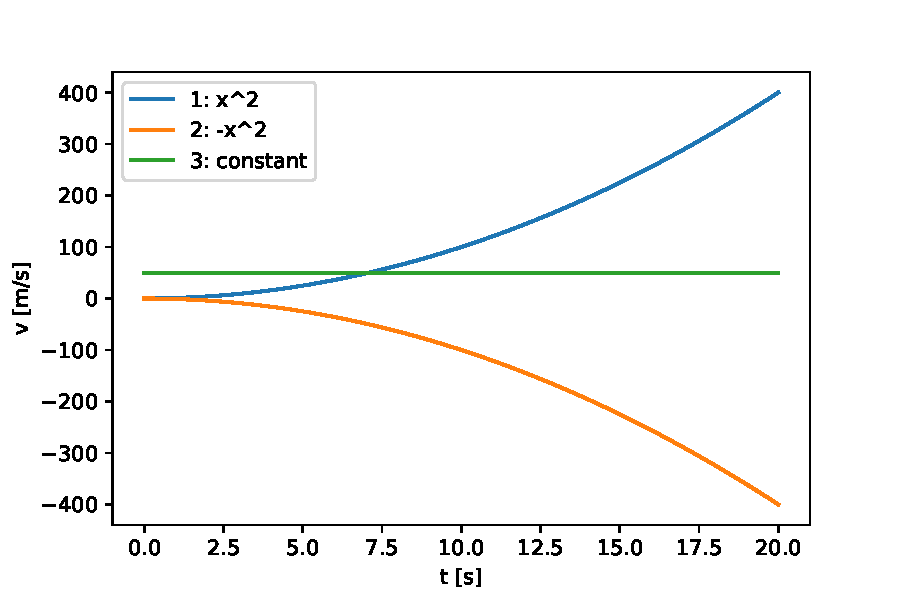
\includegraphics[width=0.8\textwidth]{Images/three_functions.pdf}
    \caption{Car velocities over time.}
    \label{fig:three_functions}
\end{figure}

\subsection{Trapezoid Rule}
Euler's method forms the basis for many numerical calculations up to and including state of the art astrophysical simulations, but, without any modifications, the basic Euler scheme described by equation \ref{eq:euler} is way too simple to work in practice. That said, small tweaks to Euler's method can work wonders with respect to accuracy. For instance, while equation \ref{eq:euler} uses the velocity at the \emph{start} of a time period, the \textbf{trapezoid rule} instead uses the \emph{average of the velocities at the start and end} of the time period. Given equation \ref{eq:vel}, the trapezoid rule therefore states that

\begin{equation} \label{eq:trapezoid}
\boxed{x(t_{i+1}) = x(t_i) + \left(\frac{v(t_{i+1}) + v(t_i)}{2}\right) \Delta t}.
\end{equation}

This equation is slightly more complicated than equation \ref{eq:euler} -- 
\begin{enumerate}[resume]
    \item How do you expect this to affect the time it takes a computer to run Euler's method vs. the time it takes to run the trapezoid method? What trade-offs do we have to make in the pursuit of more accurate numerical algorithms?
\end{enumerate}

\noindent
Let's return to our car example from Section \ref{sec:eulermethod}. The car still starts 10 meters from the house and still travels for 120 seconds, but now the car is slowly accelerating: at the start of the trip, the car is moving at 13 meters per second, but by the end of the trip, the car is moving at 20 meters per second.
\begin{enumerate}[resume]
    \item At the end of the trip, where does the trapezoid method predict our car to be? To solve this, plug $x(t_i)$, $v(t_i)$, $v(t_{i+1})$, and $\Delta t$ into equation \ref{eq:trapezoid} to find $x(t_{i+1})$.
\end{enumerate}

\noindent
Since the trapezoid rule takes into account both the starting \textit{and} ending velocities, it's more robust to non-constant velocities than is Euler's method. The trapezoid rule is still not perfect, however -- 
\begin{enumerate}[resume]
    \item Under what circumstances do you expect the trapezoid rule to give poor results? Would the Euler method also give poor results in these circumstances?
\end{enumerate}

\subsection{Methods Compared}
Now that we're experts with Euler's method and the trapezoid method, let's try to answer the following question: between Euler's method and the trapezoid method, which procedure is more accurate? To do this, we'll evaluate how well these numerical algorithms perform on a problem for which we know the exact answer. It'll be interesting to check how much better our approximations get as we vary the time step. \vspace{\baselineskip}

\noindent
Let's assume that we have some object whose exact position at time $t_{i+1}$ is given by
\begin{equation} \label{eq:analytic}
\boxed{x(t_{i+1}) = x(t_i) + \cos(t_i + \Delta t) - \cos(t_i)},
\end{equation}
where $\Delta t$ is the time step.
Let's set the starting position to be $x(t_i) = 10$ and the starting time to be $t_i = \pi / 2$. We'll model the velocity with a sine curve, $v(t) = \sin(t)$, so $v(t_i) = \sin(t_i) = \sin(\pi/2) = 1$ and $v(t_{i+1}) = \sin(t_i + \Delta t) = \sin(\pi/2 + \Delta t)$. \vspace{\baselineskip}

\noindent
\begin{enumerate}[resume]
    \item For each of the time steps in the table below:
    \begin{enumerate}
        \item Plug $x(t_i)$, $\cos(t_i + \Delta t)$, and $\cos(t_i)$ into equation \ref{eq:analytic} to calculate $x(t_{i+1})$ for the exact solution, and put these values in the ``Analytic'' column.
        \item Plug $x(t_i)$, $v(t_i)$, and $\Delta t$ into equation \ref{eq:euler} to calculate $x(t_{i+1})$ for the Euler-approximated solution, and put these values in the ``Euler'' column.
        \item Plug $x(t_i)$, $v(t_i)$, $v(t_{i+1})$ and $\Delta t$ into equation \ref{eq:trapezoid} to calculate $x(t_{i+1})$ for the trapezoid-approximated solution, and put these values in the ``Trapezoid'' column.
    \end{enumerate}
\end{enumerate}

\vspace{10 pt}
\begin{tabular}{c|c|c|c|c|c}
		Time Step & Analytic & Euler & Trapezoid & \% Error, Euler & \% Error, Trap  \\
\hline
\hline
$\Delta t = \pi/2$ & & & & & \\
\hline
$\Delta t = \pi/4$ & & & & & \\
\hline
$\Delta t = \pi/6$ & & & & & \\
\end{tabular}
\vspace{\baselineskip}

\begin{enumerate}[resume]
    \item Now, calculate the percent error of each approximate value (i.e., the ``Euler'' and ``Trapezoid'' columns) compared to the analytic value:
    \begin{equation} \label{eq:error}
    \text{\% Error} = \left|\frac{x_{\rm approx} - x_{\rm analytic}}{x_{\rm analytic}}\right| \times 100.
    \end{equation}
    Use these numbers to fill out the last two columns of the table above.
    \item How do the errors change as the time step gets smaller?
    \item Which method is more accurate when $\Delta t = \pi/2$? Which method is more accurate in general?
    \item Compute the ratio of the error from Euler's method for the longest and shortest time steps; do the same for the trapezoid method. Which method's accuracy increased more dramatically with the change in time step?
\end{enumerate}

\noindent
Euler's method and the trapezoid method are by no means the only numerical algorithms for integrating differential equations -- the literature on numerical differential equation solvers is remarkably rich, covering a myriad  algorithms differing widely in accuracy, efficiency, and stability. For further reading, you can check out \url{https://en.wikipedia.org/wiki/Numerical_methods_for_ordinary_differential_equations}.

\section{Numerical Simulations: The Double Pendulum}

Now, we can apply what we've learned about numerical algorithms to analyze a small \textbf{numerical simulation}! Numerical simulations are some of the most informative tools in modern physics and astrophysics, yet, at their core, these simulations consist of nothing more than a numerical differential equation solver integrating a bunch of equations over time and space. Usually, the systems being simulated are highly \textbf{nonlinear}, meaning that a change of the input is not proportional to the change of the output; this makes the behavior of nonlinear systems intractably difficult to follow analytically. Typically, nonlinear systems are modeled by very complex systems of coupled differential equations, thus necessitating the use of numerical approximation by a computer. \vspace{\baselineskip}

\medskip \noindent
A great example of a nonlinear system is a double pendulum. To form a double pendulum, just take one simple pendulum and connect a second one to the bottom. If you pull the pendulum a small distance from its resting place, its motion will not be periodic (repeating), but it will follow a simple, harmonic pattern -- this is \textit{linear} behavior. However, if we give the double pendulum a good kick, weird stuff starts to happen. We can model a double pendulum mathematically by tracking the angles formed by the two rods of the pendulum:
\begin{equation} \label{eq:theta1}
    \theta_1'' = \frac{-g(2m_1 + m_2)\sin\theta_1 - m_2 g \sin(\theta_1-2\theta_2) - 2\sin(\theta_1-\theta_2)m_2(\theta_2'^2 L_2 + \theta_1'^2 L_1 \cos(\theta_1-\theta_2))}{L_1 (2m_1 + m_2 - m_2\cos(2\theta_1-2\theta_2))};
\end{equation}
\begin{equation} \label{eq:theta2}
    \theta_2'' = \frac{2\sin(\theta_1-\theta_2)(\theta_1'^2 L_1(m_1 + m_2) + g(m_1 + m_2)\cos\theta_1 + \theta_2'^2 L_2 m_2 \cos(\theta_1-\theta_2))}{L_2(2m_1 + m_2 - m_2\cos(2\theta_1 - 2\theta_2))}.
\end{equation}

\medskip \noindent
Ugly!!!! Instead of worrying about analyzing these equations, let's have the computer solve them for us. Head over to this link: \url{https://myphysicslab.com/pendulum/double-pendulum-en.html} to find a simulation of a double pendulum. Follow the instructions below, recording your results in your notebook.

\begin{enumerate}
\item Wait for the program to load -- you'll need Java enabled in your browser. When the page has loaded, select the tab labeled ``graph'' in the upper left; you should then see a plot on the left side of the screen and a cartoon pendulum on the right side of the screen. Click the reset button below the plot (the button looks like a circular arrow, to the left of the play/pause button) and then click ``clear graph" below the reset button. The pendulum should be stopped in its default position and the graph should show nothing. 

\item Click and drag the bottom pendulum bob (mass 2) \textit{very} slightly to the left. Click the play button (right arrow) below the plot and observe what happens to the pendulum and what happens in the graph. Record this behavior in your notebook. Sketch the pattern of the graph. Does it form a predictable pattern? These curves are referred to as ``Lissajous curves" and consist of combinations of simple sine and cosine functions; they are the result of linear motions.

\item Let the simulation run for a bit. What is the shape of the domain in which the graph draws? What will the graph eventually look like? Sketch this in your notebook.

\item Click reset to stop the pendulum and ``clear graph'' to erase the plot. Adjust the top bob so that the rod is vertical and lift the bottom bob up until it forms a right angle with the top pendulum (the two pendulum rods should make an `L' shape); click play and record what happens to the pendulum. Concentrate only on the top bob; does it behave funny? Draw a sketch of the graph. Is it still -- more or less -- a simple/predictable pattern? What happened to the shape of the domain in which the graph draws?

\item Return to the tab that says ``Sim'' in the top left. Find the drop-down menu on the right that says ``Diff Eq Solver'' and change the option from ``Runge-Kutta'' to ``Eulers Method'' (\href{https://en.wikipedia.org/wiki/Runge\%E2\%80\%93Kutta_methods}{Runge-Kutta} integration is a more advanced variant of Euler's method). Repeat the first experiment, where we perturbed the lower bob very slightly. Qualitatively, how does the behavior of the double pendulum differ when we use Euler's method to evolve the system vs. when we use the Runge-Kutta method? Do the results from Euler's method seem physically realistic? What does this suggest about the stability of Euler's method and the robustness of Euler's method against the accumulation of error?

\item Lastly, reset the simulation once more and click the check box on the right that says ``show energy;'' this will add a bar to the top of the simulation that shows the potential, kinetic, and total energies of the system. With Euler's method enabled, perturb the lower bob slightly and observe how the total energy changes with time; reset and repeat this with the Runge-Kutta method. How does the evolution of the total energy of the system differ when we use Euler's method vs. when we use the Runge-Kutta method? How does this evolution change when we change the time step (see box labeled ``time step'' to the right of the simulation)?

\end{enumerate}

\section{Full-Scale Astrophysical Simulations} \label{sec:sims}

\medskip \noindent
Let's have a look at some real state-of-the-art astrophysical numerical simulations. Take a few minutes to look through at least \underline{three} of the following links:
\begin{itemize}
    \item The Illustris Project: \url{https://www.illustris-project.org/media/}
    \item FIRE simulations: \url{https://fire.northwestern.edu/visualizations/}
    \item The Millenium Simulation Project: \url{https://wwwmpa.mpa-garching.mpg.de/galform/virgo/millennium/}
    \item SMAUG simulations: \url{https://www.simonsfoundation.org/flatiron/center-for-computational-astrophysics/galaxy-formation/visualizations/}
    \item Black hole accretion: \url{https://jila.colorado.edu/~pja/black_hole.html}
    \item Star formation: \url{http://www.starforge.space/movies.html}
    \item Planet migration: \url{https://jila.colorado.edu/~pja/planet_migration.html}
    \item Circumplanetary disks: \url{https://people.phys.ethz.ch/~judits/#!/page_Visualization}
\end{itemize}

\begin{enumerate}
    \item Pick \textbf{one} image or video and describe what it's showing. If applicable, answer the following: What are the spatial scales of the simulation (i.e., is the simulation focused on a small planetary system? A single star? A galaxy? The entire Universe?)? What are the time scales of the simulation (seconds? Years? Billions of years?)? Why do you think the creators of this simulation decided to simulate this particular system? Could the same information that's provided by the simulation have been obtained via telescope observations? What do you think were some of the challenges involved in simulating this particular system?
\end{enumerate}

\section{Conclusions}
\begin{enumerate}
    \item Can you think of a method which would approximate the integral to a differential equation better than the Euler method or the Trapezoid method? If not, try to find one online and briefly describe this method.
    
    \item How does the size of the timestep affect the accuracy of integrators? Can you explain why?
    
    \item What limits us from putting every physical process that we know of into simulations and solving for them accurately?
    
    \item Return to your list of advantages and complications of using a computer to study the Universe that you created at the beginning of lab. Try to add three more advantages and three more shortcomings, and, wherever possible, link these points to examples from the lab. What have you learned about computation and numerical methods from this lab?
    
    \item Do you have any feedback about this lab?
    
    \item Do you have any remaining question about numerical methods?
\end{enumerate}

\end{document}
